%% LyX 2.1.1 created this file.  For more info, see http://www.lyx.org/.
%% Do not edit unless you really know what you are doing.
\documentclass[american]{article}
\usepackage[T1]{fontenc}
\usepackage[latin9]{inputenc}
\usepackage[letterpaper]{geometry}
\geometry{verbose,tmargin=2cm,bmargin=3cm,lmargin=3cm,rmargin=3cm}
\setlength{\parskip}{\smallskipamount}
\setlength{\parindent}{0pt}
\usepackage{color}
\usepackage{url}
\usepackage{amssymb}
\usepackage{graphicx}
\usepackage{babel}
\begin{document}

\title{A 16-Channel Discriminator based on the NINO Chip\\
\textcolor{red}{DRAFT}}


\author{John R.M. Annand\\
University of Glasgow}

\maketitle

\subsection{\label{sub:Introduction}Introduction}

Following the completion of the upgrade of the CEBAF accelerator the
experimental programme in Hall A will, to a large extent, use large
acceptance spectrometers designed to operate at high luminosity
\begin{itemize}
\item \textbf{\textcolor{black}{BigBite (BB)}}, equipped with new GEM trackers,
a new gas \v{C}erenkov particle ID system, a new timing hodoscope
and a refurbished electromagnetic calorimeter.
\item \textbf{\textcolor{black}{Super BigBite Spectrometer (SBS)}}, equipped
with GEM trackers and a hadron calorimeter HCAL. The detector package
of SBS is very flexible and can be optimized for proton or neutron
detection.
\item \textbf{\textcolor{black}{Electromagnetic Calorimeter}}: which is
a highly segmented lead-glass array to detect high energy electrons
or photons.
\item \textbf{\textcolor{black}{Coordinate Detector:}} a finely segmented
plastic hodoscope, intended to be used in conjunction with calorimeters,
when optimum angular resolution is required.
\end{itemize}
The GEM tracking systems will have specialist readout based on the
APV25 chip, but for fast counting detectors where amplitude and time
information are required a different approach is needed. Here a an
amplifier/discriminator card based on the NINO chip from CERN is described.
Thus far it is envisaged that the card will be used on several components
of the BB/SBS system including:
\begin{itemize}
\item GRINCH gas \v{C}erenkov 540 elements.
\item BB Timing Hodoscope 180 elements.
\item Coordinate detector 3328 elements.
\end{itemize}

\subsection{\label{sub:Description}Description of the Card}

\begin{figure}[h]
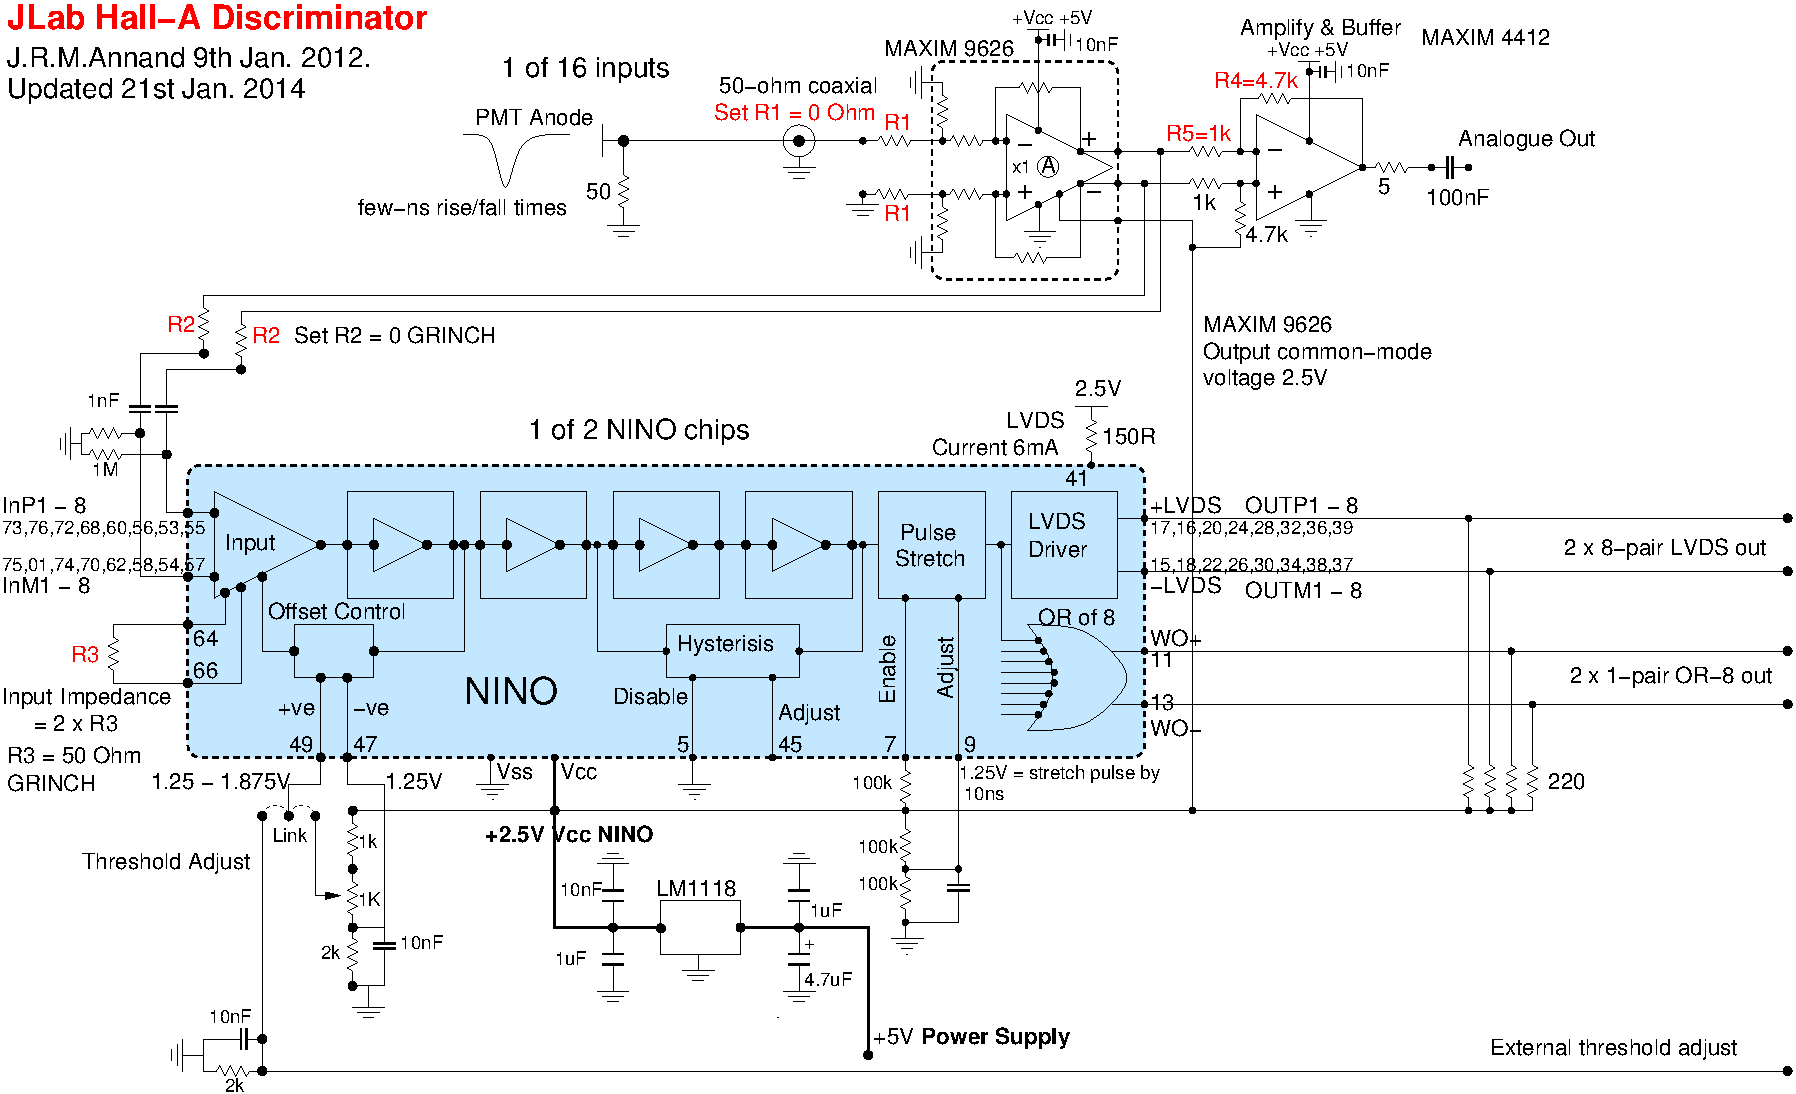
\includegraphics[width=1\columnwidth]{CherenkovNINO-4}

\protect\caption{\label{fig:nino-schematic}Circuit diagram of the discriminator card.
A schematic diagram of the NINO chip is shown in the area shaded blue.}


\end{figure}


The discriminator card (Fig. \ref{fig:nino-schematic}) is based on
the NINO chip \cite{NINO}, shown schematically in the blue-shaded
box of Fig\ref{fig:nino-schematic}. NINO was designed originally
for time of flight systems at the ALICE experiment. It is an 8-channel
CMOS ASIC which accepts differential input signals and provides LVDS
output signals for timing. The output width is dependent on the charge
of the input signal and may be stretched by an amount, dependent on
the voltage applied to pin 9. This is currently 1.25~V, which stretches
by 10~ns. The threshold is set by applying a differential DC voltage
to pins 47 and 49. Pin 47 is fixed at 1.25~V and 49 is varied between
1.25~V (zero threshold) and 1.90~V (maximum). Ref. \cite{NINO}
specifies that the threshold range is 10-100~fC and for the present
application this translates to a voltage levels in the few-mV range
(Sec.\ref{sub:Testing}). This enables PMTs to be run at moderate
gain when it is desired to detect single photoelectron pulses. When
used in conjunction with a multiple resistive plate chamber at CERN,
NINO achieves a timing resolution of around 60~ps. However with the
$\sim5$~ns rise-time pulses from the 9125 photomultipliers (PMT)
attached to the GRINCH gas \v{C}erenkov the resolution will be $\gtrsim500$~ps.
Cosmic-ray tests of the BigBite, plastic scintillator timing hodoscope,
using the NINO discriminator card, give a timing resolution of around
100~ps. In this case fast, Hamamatsu R-11265 PMT were used.

For Hall-A/SBS experiments, the discriminator card will be used with
PMT so that a front-end circuit is required to convert the input signal
from single ended to differential. This is implemented using the MAXIM
9626, which is a unity-gain, low-noise, low-distortion, fully-differential
amplifier, with a bandwidth of 1.35~GHz. Resistors R1 allow the input
impedance to be tuned to the input transmission line and for 50~$\Omega$
coaxial cable R1 = 0~$\Omega.$ The differential output from the
MAXIM 9626 feeds to the NINO input via capacitors which block the
common-mode voltage offset applied to the input circuit. Resistors
R2 can potentially be used to provide some attenuation of the pulse
(to vary the threshold range), but for GRINCH R2 = 0~$\Omega.$ Resistor
R3 sets the input impedance of NINO and the current value of 50~$\Omega$
sets the impedance to 100~$\Omega.$

The front end also provides a buffer amplifier, suitable to drive
charge digitizing hardware. This is required to calibrate the non-linear
relation between time-over-threshold and pulse amplitude. It is implemented
using the MAXIM 4412 operational amplifier, which is moderately fast
and relatively inexpensive. The gain is $(1+R4/R5)$, nominally a
factor 5.7.

Fig.\ref{fig:nino-photo} is a photograph of the Mk-IV prototype card.
Components are mounted on a 5-layer PCB, designed and manufactured
by ZOT Integrated Manufacturing (\url{http://www.zot.co.uk/}) based
in Musselburgh, Scotland. Components are surface mounted, but for
the NINO chips standard solder masking techniques did not give a reliable
connection to the PCB, due to the fine pitch of the pads. The ``balling''
technique, whereby precise quantities of solder are deposited on the
pads, solved this problem. The card is designed for stand-alone operation
(i.e. it does not reside in an electronics crate), so that it can
be mounted close to the detector using the four mounting points at
the corners of the card. The printed circuit board houses 2 Mk1 (8-channel)
NINO chips, associated front-end amplifier circuitry, connectors for
input signals and connectors for output analogue and LVDS logic signals.
Input cables can be connected, either by the $16\times2$-pin arrangement
shown in Fig.\ref{fig:nino-photo}, or alternatively hard soldered
to the card. Provision of a connector to allow cables to be routed
parallel to the plane of the card is to be implemented on future production
versions of the card. The output connectors are standard 17-pair,
0.1'' pitch IDC, commonly used with ECL logic.

The card operates from a single +5V supply which powers the operational
amplifiers and a voltage regulator which supplies 2.5~V to the NINO
chips. The amount of current drawn on the 5~V line is 1.25~A. Discriminator
thresholds can be adjusted by on-board potentiometers, or alternatively
from an external voltage source. This is chosen by the position of
the jumpers on the ``Link Ext Thr'' pins attached at the bottom
left and right of the PCB. As shown, the PCB has been configured to
operate with external voltage thresholds, supplied via the ``Thr1''
and ``Thr2'' connectors at the bottom of the card. When mounted,
the card will be covered by a metal sheet to shield from electromagnetic
disturbance and will include attachments to clamp input and output
cables in place.

\begin{figure}[h]
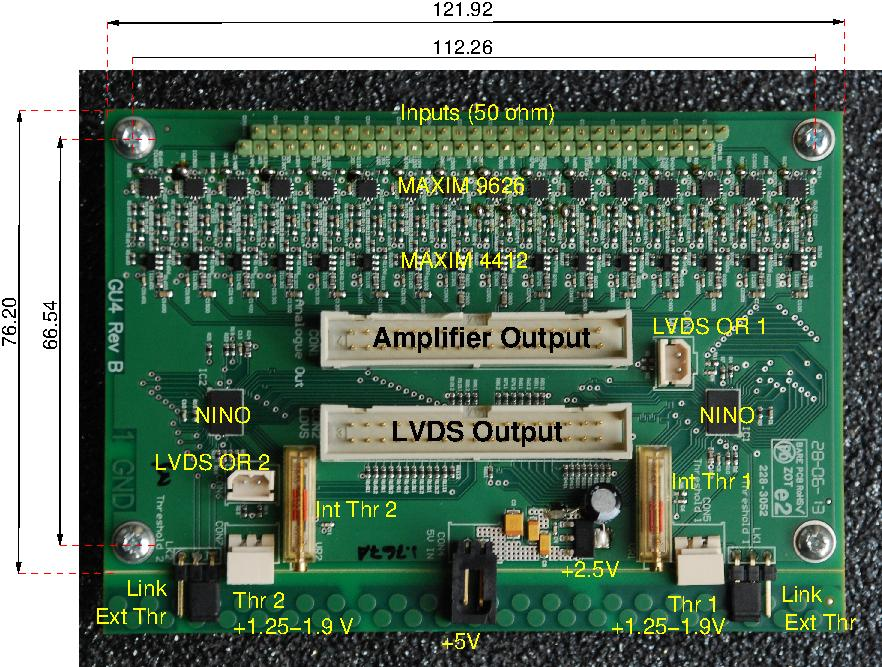
\includegraphics[width=1\columnwidth]{NinoCardPhoto}

\protect\caption{\label{fig:nino-photo}The NINO-based amplifier-discriminator card.
Dimensions are in mm. Displayed is a prototype board. GRINCH and hodoscope
cards will have type-MCX coaxial connectors.}
\end{figure}



\subsection{\label{sub:Testing}Testing of the NINO Prototype}

Preliminary testing of the NINO card has been performed using the
output from a plastic scintillator attached to a XP2262 PMT. Signals
are displayed in Fig.\ref{fig:Oscilloscope-plots}A and B. Note that
the LVDS output signal (cyan) has been obtained with an active differential
probe. Plot A corresponds to a threshold voltage of 1.3~V and the
corresponding threshold is difficult to discern on the input signal.
The amplifier output shows a threshold level of $\lesssim5$~mV,
equivalent to $\lesssim1$~mV on the input. In spite of this extremely
low level threshold the discriminator triggered cleanly on pulses
from the scintillator. Plot B shows the threshold levels for a threshold
setting of 1.9~V which corresponds to around 20~mV on the input
pulse. Plots C and D were obtained using input from a pulse generator.
Plot C displays the response to a train of pulses of amplitude around
25~mV spaced around 80~ns apart. The threshold setting was 1.5~V
and there are no losses from the discriminator. Plot D shows the double-pulse
response, with re-triggering achieved on pulses down to $\sim23$~ns
apart. The minimum re-triggering time will of course depend on the
input pulse width and the amount of stretch programmed on the NINO
chip (Sec. \ref{sub:Description}).

\begin{figure}[h]
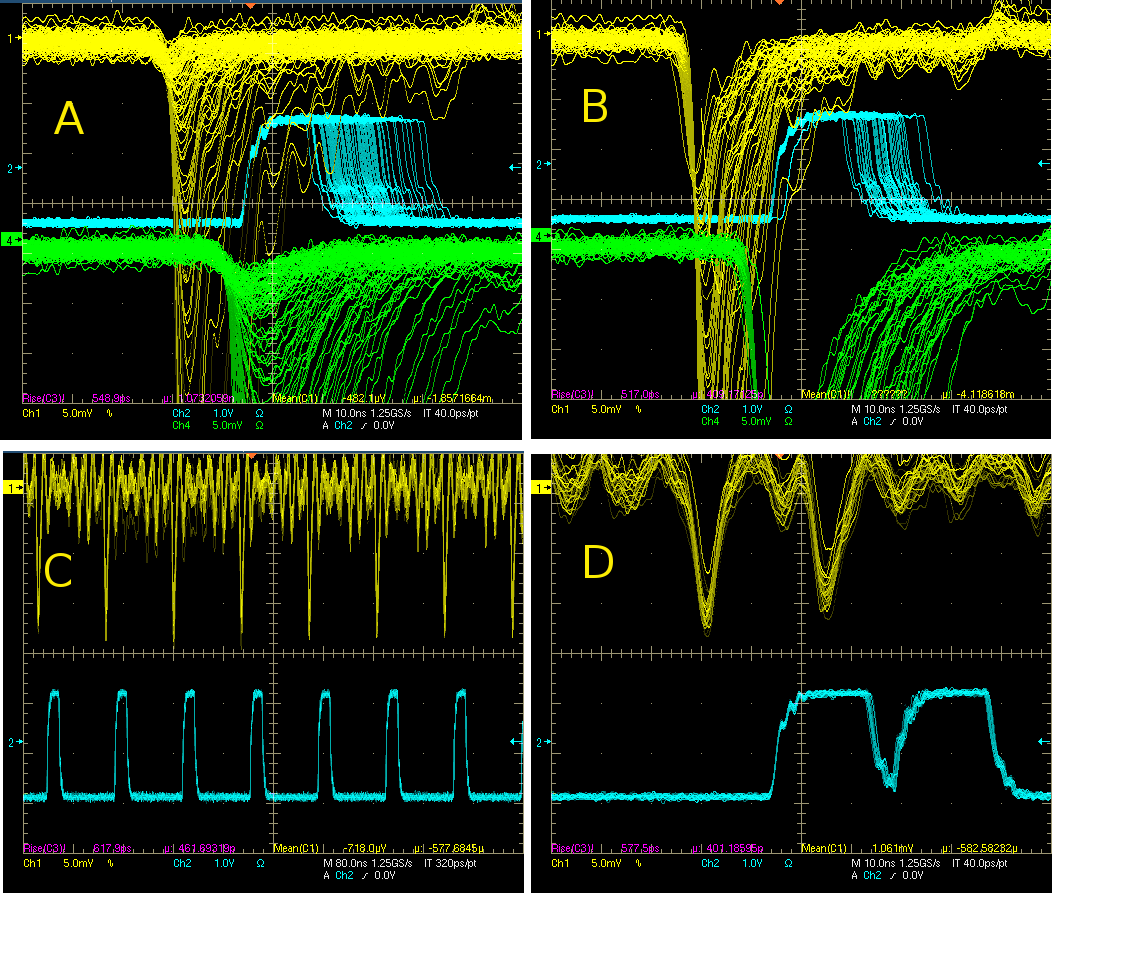
\includegraphics[width=1\columnwidth]{ninoB4}

\protect\caption{\label{fig:Oscilloscope-plots}NINO oscilloscope plots. The color
coding is yellow: input signal (5~mV per vertical division); green:
amplifier output signal (5~mV per vertical division); cyan: LVDS
logic signal (1~V per vertical division). Plots A, B and D have a
horizontal scale of 10~ns per division while plot D has 80~ns per
division. The oscilloscope was triggered by the LVDS logic signal.}


\end{figure}


The NINO card has been tested with a prototype element of the BB timing
hodoscope as shown in Fig.\ref{fig:Test-setup}. At the moment this
is equipped with relatively slow (5~ns rise time) 9125 PMTs (as will
be used on GRINCH), which limit the achievable timing resolution.
Two small plastic scintillators, placed above and below the hodoscope
bar, provide a trigger for energetic charged particles (cosmic-ray
muons). All PMT signals are passed to a NINO card and in addition
the trigger scintillator PMT outputs are split and attached to Ortec
934 CFDs which provide NIM signals to fire the DAQ system. This consists
of a VMEbus crate housing a i686-based controller running Linux, a
CAEN V1190A multi-hit TDC and a CAEN V792 QDC. The LVDS signals from
NINO are fed directly to the TDC, which has a resolution of 100~ps/channel
and has been programmed to record both the leading and trailing edges
of the LVDS pulse. The amplifier outputs from the NINO card are fed
to the QDC, which has 12-bit resolution and a full-scale limit of
400~pC.

\begin{figure}[h]
\includegraphics[width=1\columnwidth]{TestBed2a}

\protect\caption{\label{fig:Test-setup}Test setup showing one element of the BigBite
timing hodoscope, and two trigger scintillators placed above and below
the hodoscope element.}


\end{figure}


Fig. \ref{fig:Correlation1} shows the correlation of leading-edge
hit time from a single PMT of the hodoscope with the time-over-threshold
(TOT) for the same signal. TOT is just the difference of trailing-
and leading-edge recorded hits, times the TDC conversion gain of 100~ps/channel.
The correlation is smooth and quite close to linear over most of the
dynamic range, so that it can be used to correct for time walk. Fig.\ref{fig:Correl2}
shows the correlation between TOT with the charge from the buffer
amplifier, measured by the QDC. The cut-off at a TOT of 10~ns is
not completely sharp, presumably an effect of noise on very low level
input pulses. The non-linear correlation between time-over-threshold
and measured charge is smooth and ``saturates'' at a pulse charge
of around 7 units (1 unit is roughly 1~MeV energy deposit in the
hodoscope bar). The ``saturation'' corresponds to approaching the
full-scale limit of the QDC. The linear dynamic ranges of the 9125
PMT (equipped here with a redesigned low-gain/high-linearity base)
and the buffer amplifier on the NINO card remain to be quantified.
However for GRINCH operation, signal amplitudes will be well within
the linear range of the system.

\begin{figure}[h]
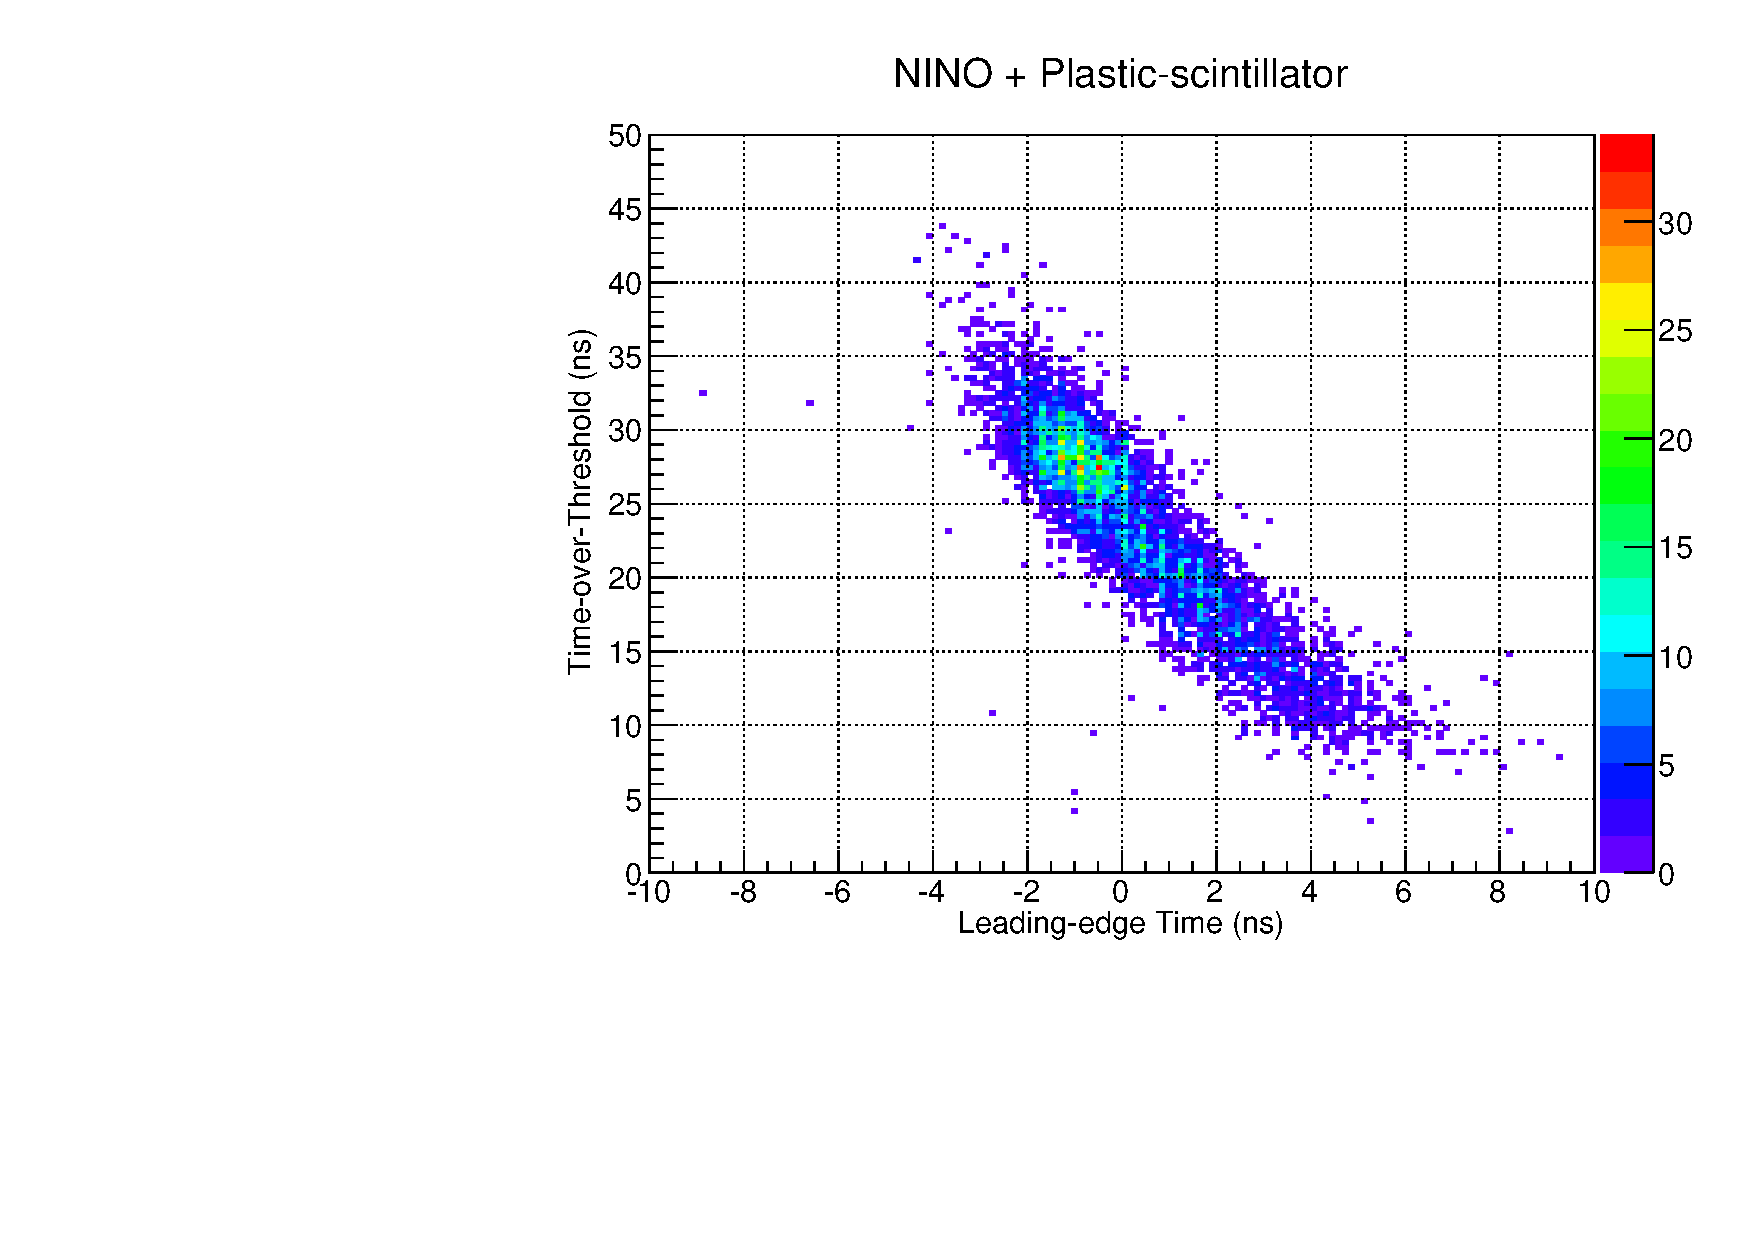
\includegraphics[width=1\columnwidth]{NinoT1}

\protect\caption{\label{fig:Correlation1}Correlation of NINO leading edge time with
time over threshold}


\end{figure}


\begin{figure}[h]
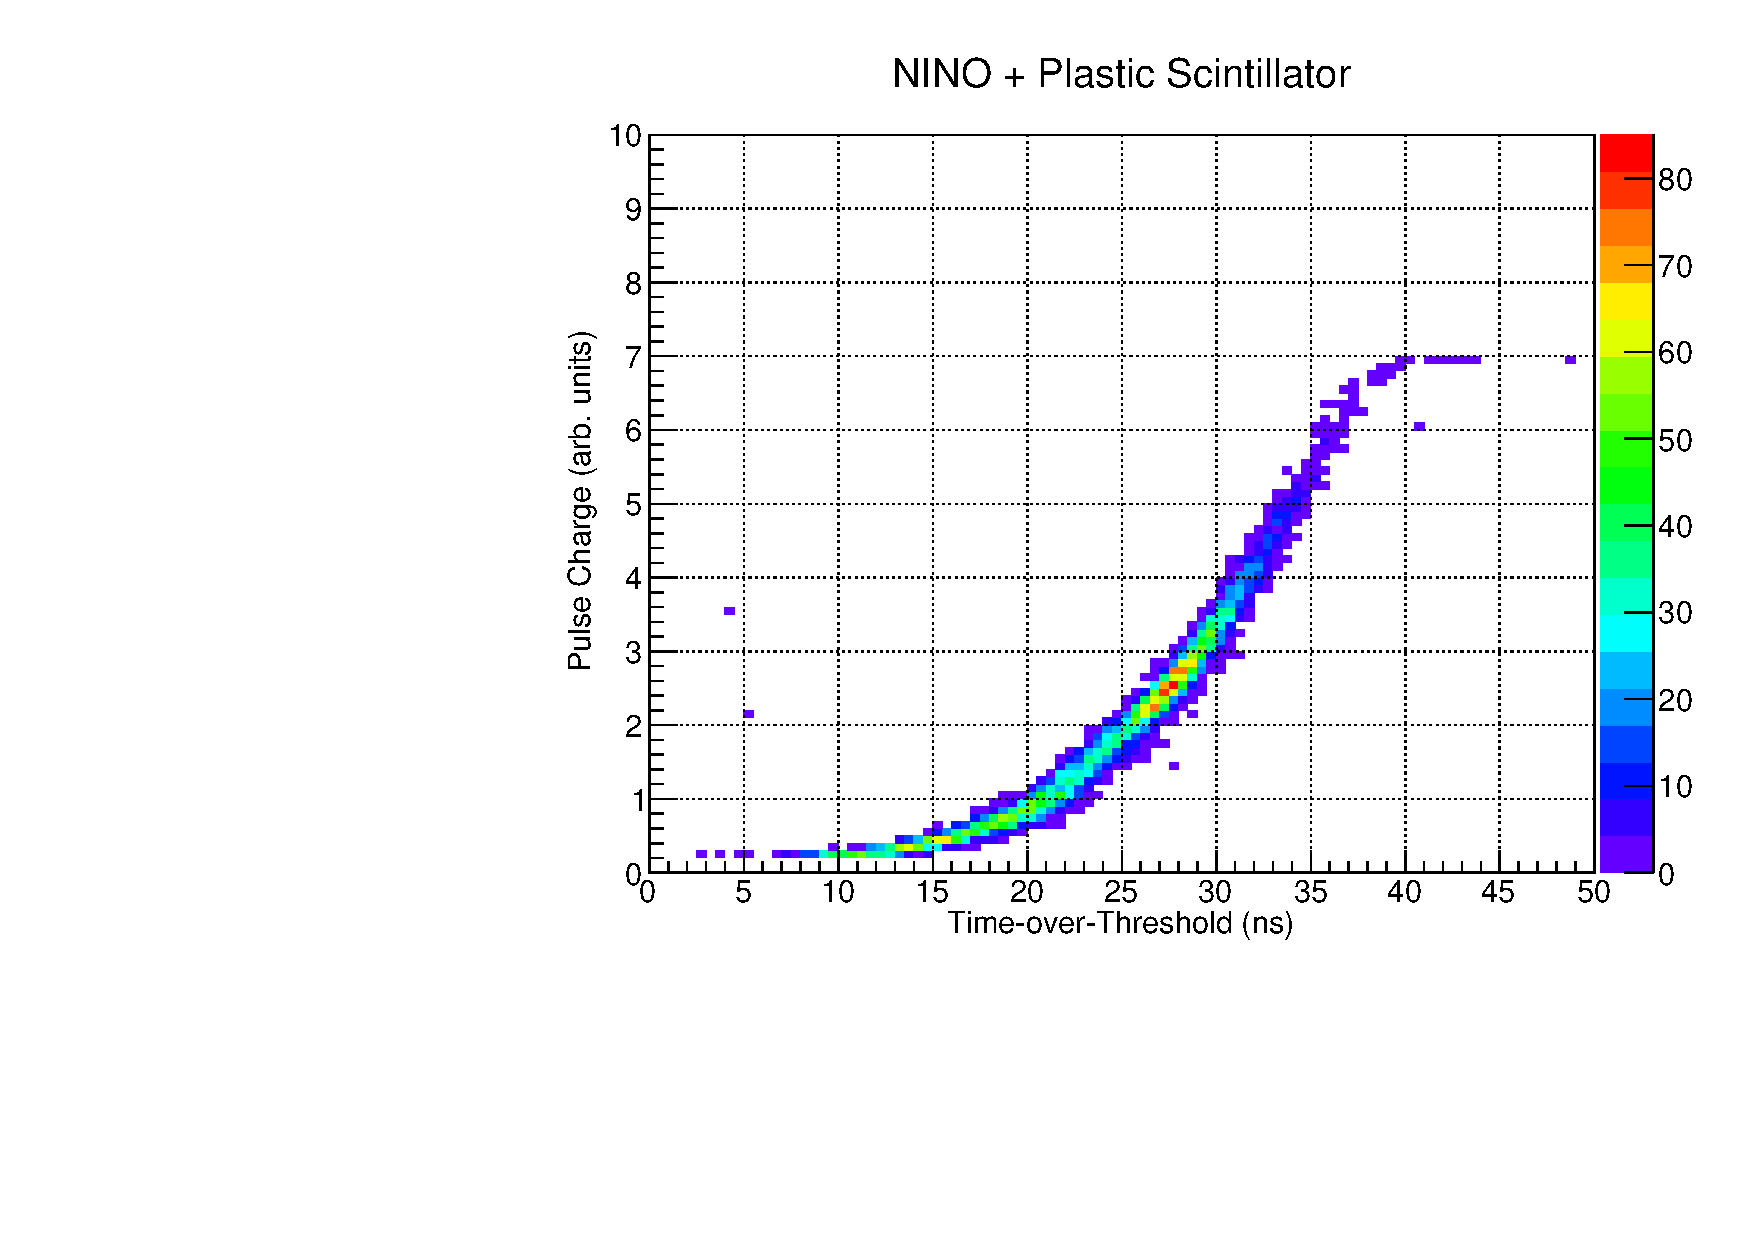
\includegraphics[width=1\columnwidth]{NinoT2}

\protect\caption{\label{fig:Correl2}Correlation of NINO time over threshold with the
pulse charge measured in a V792 QDC. Y-axis ``arb. units'' are approximately
deposited energy in MeV.}


\end{figure}

\begin{thebibliography}{1}
\bibitem{NINO}F. Anghinolfi et al., Nucl. Instr. and Meth. A 533
(2004), 183.\end{thebibliography}

\end{document}
